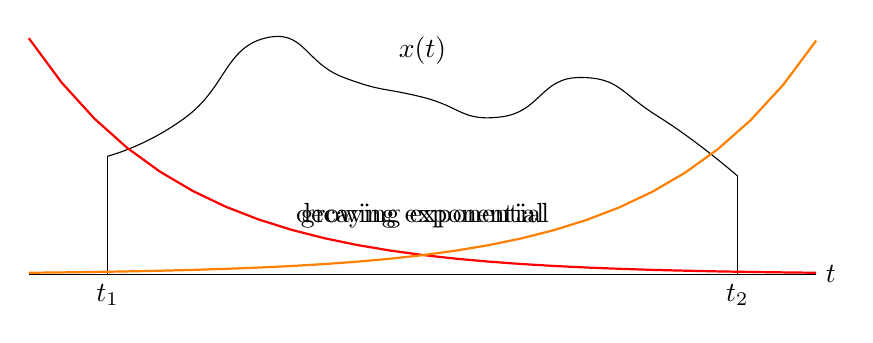
\begin{tikzpicture}[scale=1]
\draw (-5,0) -- (5,0) node[anchor=west] {$t$};
\draw  plot[smooth, tension=0.9] coordinates {(-4,1.5) (-3,2)(-2,3) (-1,2.5) (0,2.25) (1,2) (2,2.5) (3,2) (4,1.25)} node[midway, anchor=south, yshift=1in] {$x(t)$};
\draw (-4, 1.5) -- (-4, 0) node[anchor=north] {$t_1$}  (4,1.25) -- (4, 0) node[anchor=north] {$t_2$} ;
\onslide<2>
{
    \draw[thick, red,domain=0:10] plot({\x-5},{3*exp(-\x/2)}) node[midway, anchor=south, yshift=3ex, black] {decaying exponential};
}
\onslide<3->
{
    \draw[thick, orange,domain=0:10] plot({\x-5},{(exp(\x/2))/50}) node[midway, anchor=south, yshift=3ex, black] {growing exponential};
}
\end{tikzpicture} 